\subsubsection{Platforme utilisables pour garantir le fonctionnement de nos algorithmes}

Malgré que nos algorithmes aient pour but d'être déployer sur l'environnement interne de Thales SE-STAR, il nous a fallut trouvé des environnement suffisamment complexe pour tester la robustesse de nos agent mais aussi suffisamment simple pour ne pas devoir un temps infiniment long pour avoir notre réponse. De plus, la connection de nos algorithmes avec SE-STAR est un enjeu essentielle et a apporté son lot de difficulté. Il n'était donc pas raisonnable d'attendre ni de tester nos agents sur cette plateforme.

Il existe de nombreuses plateformes dédiées à l'apprentissage par renforcement. Nous avons choisis de nous concentrer sur des environnements proches de SE-STAR. Ainsi, de nombreuses études en RL utilise des jeux Atari en 2D et 3D. Nous allons donc nous basé en partie sur ce type d'environnement.

Vous pouvez voir page suivante plusieurs types d'environnements sur des plateformes différentes:

\begin{enumerate}
    \item \textbf{Gym\cite{1606.01540} - OpenAI}\\
    Gym est une plateforme qui met à disposition des jeux Atari et des simulations typiques en contrôle (Cartpole, MountainCar ...). La plateforme fournit une API permettant de réutiliser nos codes sur l'ensemble des simulations qui sont fournis par Gym.
    
    L'API de Gym étant simple, nous avons décider de nous basé sur cette API pour la construction d'un wrapper autour de la simulation interne de Thales SE-STAR.
    
    \item \textbf{Universe - OpenAI}\\
    Universe est une autre plateforme mettant à disposition une multitude de jeux très différents les uns des autres (2D, 3D, textes ...). Certains sont récents et demande une certaines réflexions (Portal, age of empire, ...). l'organisation de Universe est plus complexe que celle de gym et impose la prise en compte de plus d'éléments (réseau, possible lag, infrastructure ...). 
    
    Universe propose donc des environnements plus difficiles à tout point de vue que Gym néanmois cette plateforme n'est pas encore utilisé par les chercheurs et on peut douter de la maintenance du projet Universe (OpenAI semble mettre en avant Gym)
    
    \item \textbf{DeepmindLab\cite{DBLP:journals/corr/BeattieLTWWKLGV16} - Deepmind / Google }\\
    Le deepmindlab est une seul simulation de labyrinthe 3D très proche de notre application. Le problème est la difficulté d'utilisation de cette plateforme. Ainsi, nous n'avons pas utilisé cette ressource néanmoins elle est pertinant et est une cible pour tester nos algorithmes.
    
    \item \textbf{Doom - Vizdoom\cite{DBLP:journals/corr/KempkaWRTJ16}  }\\
    Doom est un jeu PC de tir à la première personne. Cet environnement est devenu un classique dans la communauté RL pour tester les algorithmes. A tel point que l'université de Poznan à créer une compétition d'IA basée sur Doom. L'intérêt de ce environnement contrairement au précédant et qu'il est plus complet avec un ensemble d'actions possibles conséquent. De plus, l'environnement de Doom met en lumière des difficulté pour les IA en matière d'exploration de l'environnement et est donc un terrain de jeu pour résoudre ou proposer des algorithmes résolvant ce type de problème.
    

\end{enumerate}

\bigskip
\begin{figure}
\centering
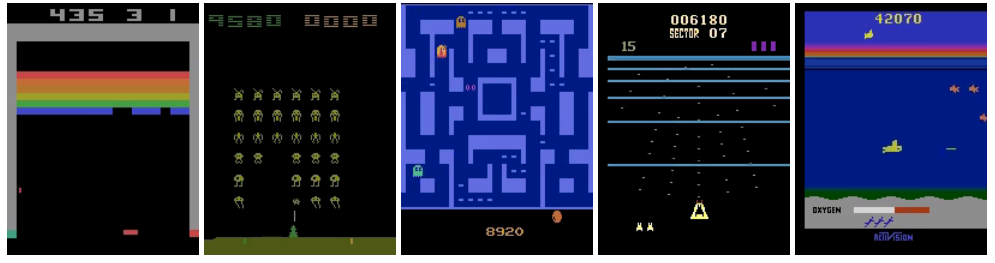
\includegraphics[width=.9\linewidth]{./assets/GYM/gym2}
\caption{Exemple d'environnements GYM (Open AI)}

\bigskip

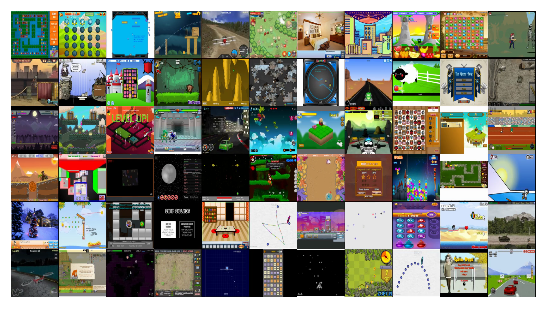
\includegraphics[width=.9\linewidth]{./assets/GYM/gym}
\caption{Exemple d'environnements Universe (Open AI)}

\bigskip

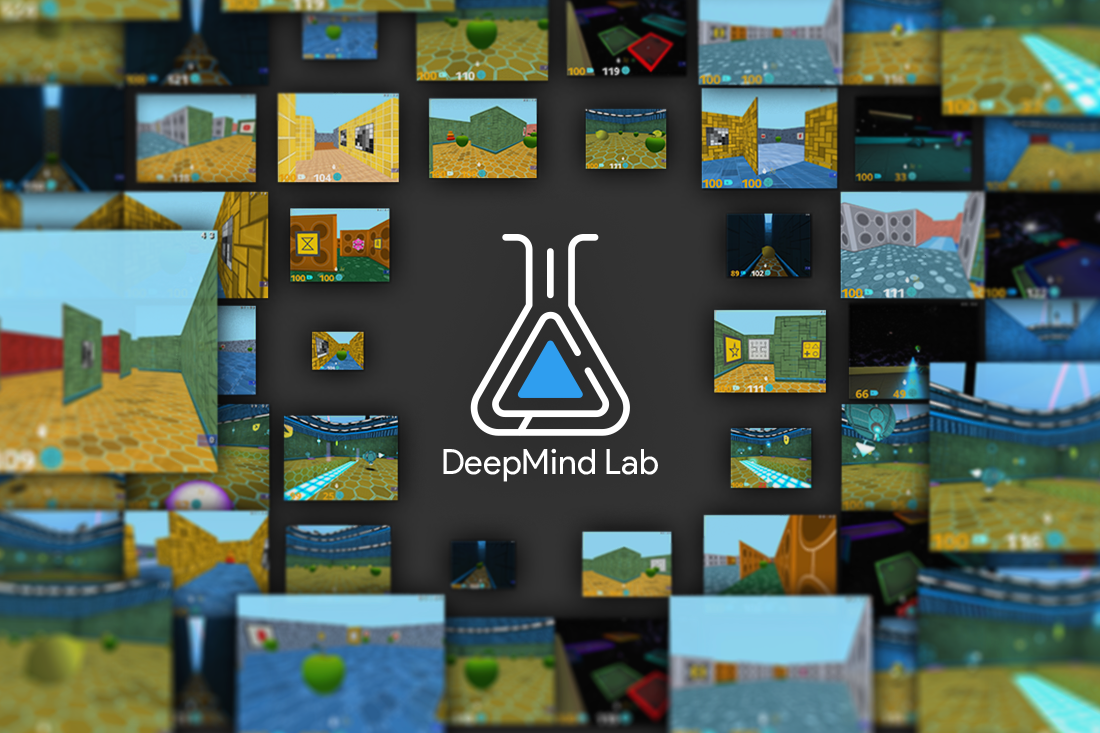
\includegraphics[width=.6\linewidth]{./assets/GYM/deepmindlab}
\caption{Exemple d'environnements DeepmindLab (Deepmind (Google)) }
\medskip
\small
\end{figure}


